\documentclass[border=10pt]{standalone}

\usepackage{tikz}
\usepackage{tikzsymbols}
\usetikzlibrary{calc,patterns,shapes.geometric}

\def\centerarc[#1](#2)(#3:#4:#5){\draw[#1] ($(#2)+({#5*cos(#3)},{#5*sin(#3)})$) arc (#3:#4:#5);}

\begin{document}
	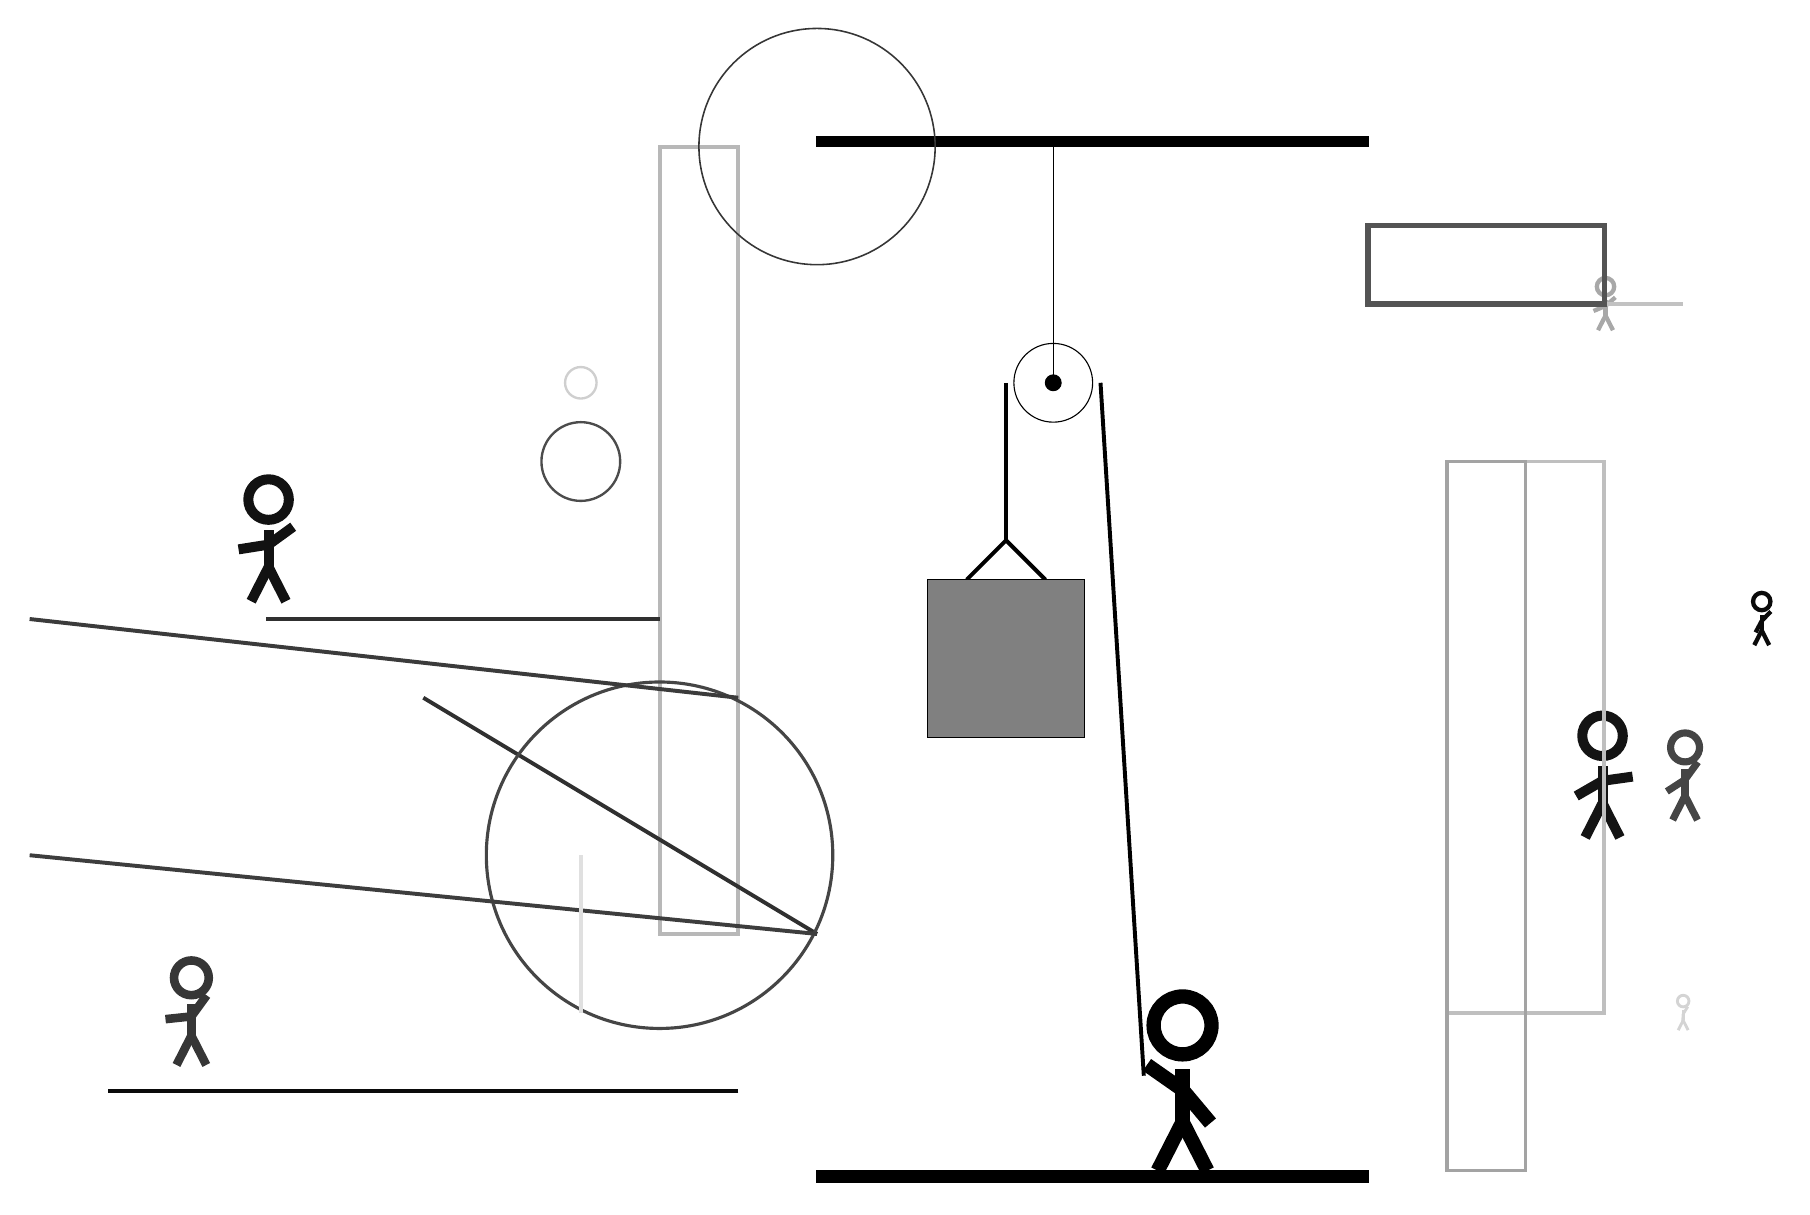
\begin{tikzpicture}
		%%%%% START %%%%%
		
		\draw[fill=black] (-2, 10) rectangle (5, 10.125);
		
		\draw[line width=0.5mm, color=black!28] (-4, 10) rectangle (-3, 0);
		
		\node[line width=0.5mm, color=black!73] at (9, 2) {\Strichmaxerl[5][33][54]};
		\draw [line width=0.2mm, color=black!79](-2, 10) circle (1.5);
		\draw[line width=0.5mm, color=black!81](-7, 3) -- (-2, 0);
		\draw [line width=0.4mm, color=black!73](-4, 1) circle (2.2);
		
		\node[line width=0.3mm, color=black!92] at (8, 2) {\Strichmaxerl[7][30][8]};
		\node[line width=0.7mm, color=black!79] at (-10, -1) {\Strichmaxerl[6][6][54]};
		\draw[line width=0.5mm, color=black!25] (6, -1) rectangle (8, 6);
		\draw [line width=0.3mm, color=black!70](-5, 6) circle (0.5);
		
		\node[line width=0.6mm, color=black!96] at (10, 4) {\Strichmaxerl[3][62][46]};
		\draw[line width=0.5mm, color=black!96](-3, -2) -- (-11, -2);
		\node[line width=0.5mm, color=black!34] at (8, 8) {\Strichmaxerl[3][23][41]};
		\draw[line width=0.5mm, color=black!81](-4, 4) -- (-9, 4);
		
		\node[line width=0.2mm, color=black!17] at (9, -1) {\Strichmaxerl[2][86][58]};
		\draw [line width=0.3mm, color=black!19](-5, 7) circle (0.2);
		\draw[line width=0.5mm, color=black!24](8, 8) -- (9, 8);
		\node[line width=0.3mm, color=black!93] at (-9, 5) {\Strichmaxerl[7][9][36]};
		
		\draw[line width=0.4mm, color=black!36] (7, 6) rectangle (6, -3);
		\draw[line width=0.5mm, color=black!76](-2, 0) -- (-12, 1);
		
		\draw[line width=0.5mm, color=black!12](-5, -1) -- (-5, 1);
		\draw[line width=0.5mm, color=black!77](-3, 3) -- (-12, 4);
		\draw[line width=0.7mm, color=black!67] (5, 8) rectangle (8, 9);
		
		\draw (1, 7) circle (0.5);
		\draw[fill=black] (1, 7) circle (0.1);
		\draw (1, 10) -- (1, 7);
		
		\draw[line width=0.5mm] (-0.1, 4.5) -- (0.4, 5.0) -- (0.9, 4.5);
		\draw[fill=black!50] (-0.6, 4.5) rectangle (1.4, 2.5);
		
		\draw[line width=0.5mm] (0.4, 7) -- (0.4, 5.0);
		\centerarc[line width=0.5mm](1, 7)(0:180:0.6);
		\draw[line width=0.5mm](1.6, 7) -- (2.15, -1.8);
		
		\node at (2.6, -1.9) {\Strichmaxerl[10][-35][-50]};
		
		\draw[fill=black] (-2, -3) rectangle (5, -3.15);
		
		%%%%% END %%%%%
	\end{tikzpicture}
\end{document}